\documentclass{article}

\usepackage[nonatbib,preprint]{neurips}
\usepackage[numbers]{natbib}

\usepackage[utf8]{inputenc}
\usepackage[T1]{fontenc}
\usepackage{microtype}
\usepackage{booktabs}
\usepackage{graphicx}
\usepackage{amsmath}
\usepackage{xcolor}
\usepackage{tikz}
\usetikzlibrary{arrows.meta,positioning,calc}
\usepackage{hyperref}
\hypersetup{colorlinks=true, linkcolor=somink, citecolor=somblue, urlcolor=somblue}

\definecolor{sombase}{HTML}{8C8C8C}
\definecolor{somblue}{HTML}{0072B2}
\definecolor{somverm}{HTML}{D55E00}
\definecolor{somgreen}{HTML}{009E73}
\definecolor{somink}{HTML}{2C3E50}
\definecolor{sompale}{HTML}{F2F4F7}

\makeatletter
\renewcommand{\@noticestring}{%
  Technical report, July 2026. Code, adapters, datasets, and run evidence:
  \url{https://github.com/AbdelStark/sommelier}%
}
\makeatother

\newcommand{\sommelier}{Sommelier}
\newcommand{\basemodel}{\texttt{Llama-3.1-Nemotron-Nano-8B-v1}}

\title{\sommelier: An Auditable Data Flywheel for\\Sovereign Tool Calling on a Single GPU}

\author{%
  Abdelhamid Bakhta\\
  \texttt{abdel@starkware.co}\\
  \texttt{github.com/AbdelStark}\\
}

\begin{document}

\maketitle

\begin{abstract}
Selecting the right tool and filling its arguments is the atomic skill of agentic AI: every plan, every multi-step workflow, every autonomous loop decomposes into this one act, repeated thousands of times. We present \sommelier, an open pipeline that post-trains a small open-weight model into a reliable tool caller and, more importantly, measures the improvement under a protocol built so that an invalid comparison refuses to exist and every failure leaves evidence. We take a position: the data flywheel, the loop in which usage produces data, data produces a better model, and a better model produces more usage, is the operational unit of AI progress, and it compounds errors exactly as fast as it compounds capability unless every turn is auditable. Sovereignty, in turn, is the measured ability to turn this flywheel yourself, on open weights, with open recipes, at a cost you can state. We report two full turns. Turn one applies QLoRA to \basemodel{} on 15{,}000 single-call examples for about three hours on one rented L40S, roughly eight dollars of GPU time, and lifts full-call exact match from 0.705 to 0.874 on 1{,}000 held-out prompts, with valid JSON reaching 1.000, under a protocol whose comparison report refuses to exist unless base and adapter were scored on digest-identical prompts, parser, and decoding. Turn two consumes turn one's published artifacts: constrained machine translation of the queries, with tool schemas and gold answers held byte-identical, moves the historical marginal full-slice difference from $-4.2$ points to $+0.3$ while English moves at most 0.8 points, within one standard error. Because the French and English slices contain 879 and 1{,}000 rows, that cross-language contrast is descriptive rather than an exact paired estimate. The published splits and aggregate reports expose checksums, numerators, denominators, and run identities sufficient to check the reported rates; raw generations were retained by the runs but are absent from the published v1/v2 repositories, so independent row-wise rescoring is not possible from those repositories alone. The dollar costs are a maintainer billing-console observation and an explicitly labeled extrapolation, not checksummed run evidence. We describe the pipeline as a set of reusable recipes, including the evaluation-design failure that nearly inverted our conclusions, and argue that this discipline is what makes small-model sovereignty real rather than aspirational.
\end{abstract}

\section{Introduction}
\label{sec:intro}

A sommelier does one thing supremely well: from a long list, select the one right option and pair it with the right accompaniments. That is precisely the job a model performs inside an agentic system. Given a request and a list of available tools, it must select the right tool and fill the right arguments. If the call is wrong, nothing downstream can save it. If it is right, cheap, and fast, everything downstream compounds.

Most teams today buy this skill by the token from a frontier API. That is a reasonable way to start and a risky way to live: the provider can reprice the model, retire it, or gate access, and none of those decisions are yours. The alternative, owning a small model tuned to your own tools, has been technically possible for years, but it comes with a credibility problem. Fine-tuning writeups typically ask the reader to trust a table. The baseline may have been prompted differently, parsed leniently, or evaluated on prompts the training set leaked into, and nothing in the table shows it.

\sommelier{} is built on the opposite premise: \emph{a fine-tuning claim is only as good as its evidence}. It is a six-stage pipeline in which stages communicate only through schema-versioned, SHA-256-checksummed files, evaluation prompts carry digests, the parser never repairs model output, and the final base-versus-adapter report refuses to exist unless both sides provably used identical data, prompts, parser, and decoding. The pipeline is MIT licensed, keeps its core GPU-free (the deterministic stages and the test suite run on a laptop with no accounts), and produced two published training runs whose aggregate reports expose metric numerators, denominators, and identity digests. The public repositories do not contain the retained raw generations, so they support checking the reported aggregates but not independent row-wise rescoring.

This paper uses those two runs to argue three things.

\begin{itemize}
  \item \textbf{Position: the flywheel is the product} (Section~\ref{sec:flywheel}). The data flywheel~\citep{nvidia2026flywheel} is the right mental model for applied AI, but the property that makes it compound in your favor is auditability. A flywheel with undeclared filters, unversioned prompts, or repair-happy parsers amplifies its own approximations on every turn. We demonstrate a flywheel whose second turn consumed the first turn's published artifacts, row by row, with provenance.
  \item \textbf{Position: sovereignty is operational, and it now has a price tag} (Section~\ref{sec:sovereignty}). Sovereignty over a tool-calling model, for one task, accompanied a maintainer-observed bill of about eight dollars, three hours of GPU time, and a pipeline you can read in an afternoon. The second turn's roughly sixteen-dollar figure is an extrapolation from that observed rate over its recorded runtime, not provider billing exposed to the run. We argue this reframes sovereign AI~\citep{singh2025sovereignai,srivastava2024digitalsovereignty,nvidia2024sovereignai} from infrastructure policy to weekend engineering, and we measure a dependency that policy discussions rarely quantify: language. In the historical unequal full slices, the base model's French rate is 4.2 points below English; the v2 artifacts do not identify that marginal difference as an exact paired language effect.
  \item \textbf{Measurements and recipes} (Sections~\ref{sec:pipeline} to~\ref{sec:recipes}). We report the complete method and results of both runs, with numerators and denominators, and we document the failure modes that a green suite of roughly 300 tests did not catch, including the evaluation-design collision that made a byte-perfect model score zero. These recipes are the educational payload of the paper: the gap between ``the tests pass'' and ``the measurement is honest'' is where most applied fine-tuning effort actually goes.
\end{itemize}

\begin{figure}[t]
  \centering
  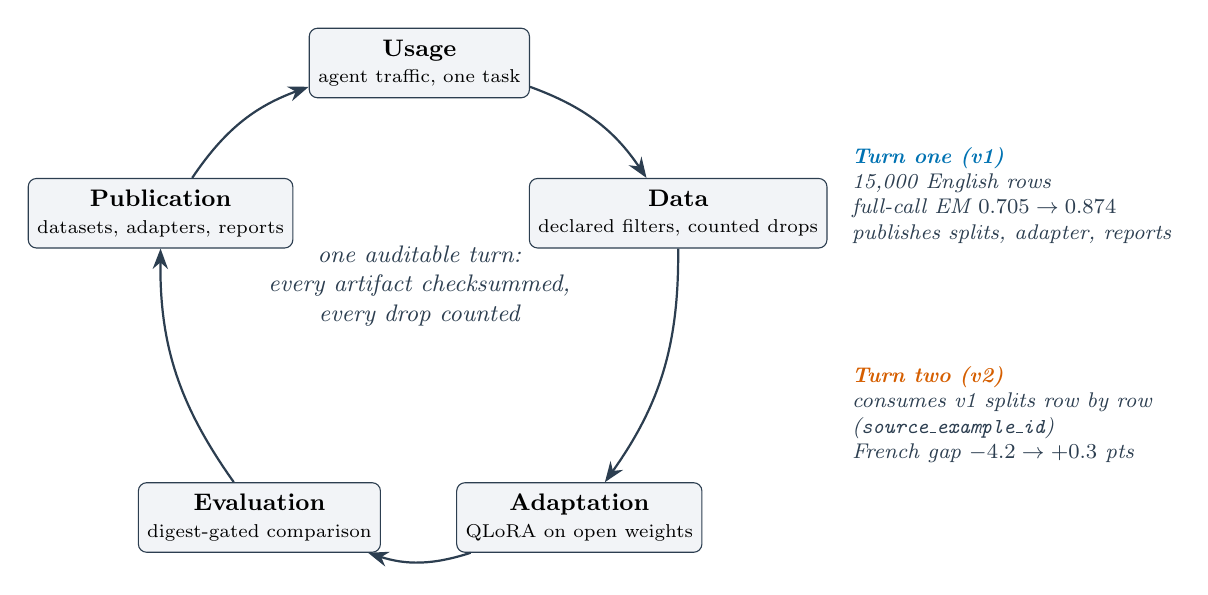
\begin{tikzpicture}[
      scale=0.96, every node/.style={transform shape},
      stage/.style={draw=somink, fill=sompale, rounded corners=3pt, align=center,
                    minimum width=2.85cm, minimum height=0.92cm, font=\small},
      turn/.style={font=\footnotesize\itshape, text=somink, align=left},
      arr/.style={-{Stealth[length=2.6mm]}, thick, somink}]
    \node[stage] (usage)   at (90:3.1)   {\textbf{Usage}\\[-1pt]\scriptsize agent traffic, one task};
    \node[stage] (data)    at (18:3.6)   {\textbf{Data}\\[-1pt]\scriptsize declared filters, counted drops};
    \node[stage] (adapt)   at (-54:3.6)  {\textbf{Adaptation}\\[-1pt]\scriptsize QLoRA on open weights};
    \node[stage] (eval)    at (-126:3.6) {\textbf{Evaluation}\\[-1pt]\scriptsize digest-gated comparison};
    \node[stage] (publish) at (162:3.6)  {\textbf{Publication}\\[-1pt]\scriptsize datasets, adapters, reports};
    \draw[arr] (usage) to[bend left=18] (data);
    \draw[arr] (data) to[bend left=18] (adapt);
    \draw[arr] (adapt) to[bend left=18] (eval);
    \draw[arr] (eval) to[bend left=18] (publish);
    \draw[arr] (publish) to[bend left=18] (usage);
    \node[align=center, font=\small\itshape, text=somink] at (0,0.15)
      {one auditable turn:\\every artifact checksummed,\\every drop counted};
    \node[turn, anchor=west] at (5.6,1.35)
      {\textbf{\textcolor{somblue}{Turn one (v1)}}\\
       15{,}000 English rows\\
       full-call EM $0.705 \rightarrow 0.874$\\
       publishes splits, adapter, reports};
    \node[turn, anchor=west] at (5.6,-1.55)
      {\textbf{\textcolor{somverm}{Turn two (v2)}}\\
       consumes v1 splits row by row\\
       (\texttt{source\_example\_id})\\
       French gap $-4.2 \rightarrow +0.3$ pts};
  \end{tikzpicture}
  \caption{The \sommelier{} flywheel. Each turn moves through usage, declared data work, adaptation, gated evaluation, and publication with provenance. The second turn consumed the first turn's published artifacts directly: every French training row names the English row it derives from, and the English evaluation prompts of both turns are byte-identical by digest.}
  \label{fig:flywheel}
\end{figure}

\section{Position: the flywheel is the product}
\label{sec:flywheel}

NVIDIA defines a data flywheel as ``a self-improving loop where data collected from AI interactions or processes is used to continuously refine AI models, generating better outcomes and more valuable data for continued improvement''~\citep{nvidia2026flywheel}. The enterprise pitch is compelling: route real traffic into curation, customization, evaluation, and redeployment, and smaller, cheaper models progressively absorb work that once required frontier-scale ones. NVIDIA reports that flywheel deployments have in some cases cut inference costs by over 98\% without accuracy loss~\citep{nvidia2026flywheel}, and its NeMo microservices demonstration fine-tunes a 1B Llama model on the same function-calling dataset we use here to approach the tool-calling accuracy of a model seventy times its size~\citep{verma2025flywheel}.

We agree with the mechanism and want to sharpen the premise. A flywheel is a feedback loop, and feedback loops do not distinguish between signal and error: they compound whatever you feed them. If the curation step applies filters nobody recorded, the next turn trains on a distribution nobody can state. If the evaluation prompt set drifts between the baseline and the candidate, the next turn optimizes against a comparison that was never valid. If the parser silently repairs malformed output, the next turn inherits a capability estimate that belongs partly to the harness. None of these failures announce themselves; each looks like a clean number in a table. This is the classic hidden-debt structure of ML systems~\citep{sculley2015hidden}, but the flywheel gives it a gear ratio.

The position of this paper is that \emph{auditability is the load-bearing property of a data flywheel}, ahead of automation and ahead of scale. Concretely, a turn of the wheel is auditable when four things hold. First, data transformations are declared and counted: \sommelier's preparation stage classifies every dropped row under one of sixteen closed drop reasons, and the drop summary is a published artifact, so ``52.6\% of source rows were filtered as multi-call'' is a statement of record, not folklore. Second, identity is checked, not assumed: every rendered prompt carries a SHA-256 digest, and the comparison gate refuses to write a report unless base and adapter evaluations agree on config digest, test-split digest, prompt-set digest, parser version, and decoding settings. Third, failures are loud: a stage that cannot meet its contract exits with an error naming the config field at fault, because a plausible-looking wrong number is strictly worse than a dead run. Fourth, publication carries provenance: what ships is not a score but a directory of checksummed files from which the score can be recomputed.

Our two runs are two turns of this wheel (Figure~\ref{fig:flywheel}), and the coupling between them is the demonstration. Turn one published its exact train/validation/test rows, its adapter, and its evaluation reports. Turn two consumed those artifacts as raw material: each French training row was produced by constrained translation of a specific published English row and carries that row's identifier (\texttt{source\_example\_id}), inherits its split assignment so translation can never leak test content into training, and must reproduce the English row's tool schemas and gold answers byte for byte. The English prompt set of turn two is digest-identical to turn one's, so the two turns are anchored to the same measurement surface. Nothing in this loop is owned by a third party; the next turn can start tomorrow morning from what turn two published. The engineering lesson we take from actually turning the wheel twice: data with unknown filters is an unusable starting point, pairs dropped without a counter are an invisible bias, and an evaluation without digests is an ambiance number. Make each turn auditable, or the next turn inherits and amplifies your approximations.

\section{Position: sovereignty is an operational property}
\label{sec:sovereignty}

Sovereign AI is usually discussed at the scale of nations: domestic compute, domestic data, domestic talent~\citep{nvidia2024sovereignai,singh2025sovereignai}. The regulatory frame, in Europe most concretely the AI Act~\citep{europeanunion2024aiact}, treats it as a matter of governance~\citep{srivastava2024digitalsovereignty}. We propose a complementary definition at the scale of a single engineering team, because that is where the dependency is actually experienced:

\begin{quote}
\emph{Sovereignty is the concrete ability to take open weights, apply open recipes, run accessible tooling, and produce a model you control, tuned to your task, on your terms.}
\end{quote}

The motivating scenario for \sommelier{} is a simulated AI-native French company that serves agentic infrastructure to its users and wants to improve accuracy and reduce cost. Its clients write in French; its agents pick tools thousands of times a day. Building on a closed hosted model, this company accepts four dependencies it cannot negotiate. The provider can change prices. The provider can retire the model: agent behavior tuned against one checkpoint does not automatically survive its replacement, and the project's source materials document contemporary instances of rapid model retirements and of access conditions ranging from identity verification to license terms excluding EU-domiciled entities from at least one major open-weights release. The provider can condition access. And, least discussed, the model's language distribution is not the company's: a model built and evaluated English-first works measurably less well in French. Before this project that last dependency was an intuition. It is now a number: on identical tools, identical gold calls, and an identical parser, with only the query language changed, the base model loses 4.2 points of full-call exact match on French input (Section~\ref{sec:turn2}). If your product lives in French, that degradation is structural, silent, and beyond your leverage as long as the model belongs to someone else.

What makes the operational definition of sovereignty non-aspirational in 2026 is that every ingredient is public, and the deepest layer is more open than most builders realize. Open weights tell you what a model is. Open recipes tell you how it came to be, and let you rerun the process. The Nemotron family illustrates the full stack: open weights across sizes~\citep{bercovich2025llamanemotron}, open post-training data, open tooling (NeMo Curator~\citep{nvidia2025nemocurator}), and, most strikingly, the actual data curation pipeline behind Nemotron-CC published end to end~\citep{nvidia2025nemotroncc}. Not a paper describing the pipeline: the pipeline. \sommelier{} is an attempt to build on that stack at the smallest useful scale and to test the promise on the task that matters most for agents. The interests here align openly: the vendor of accelerated computing gains when a thousand teams run their own post-training, and the teams gain models they own. For the French company, the operational conclusion fits in one sentence: the shovels are for rent, the model stays yours.

After two turns of the flywheel we can state what sovereignty over one narrow capability costs. Turn one: about eight dollars of GPU time and three hours on one rented L40S. Turn two, which added a second language: roughly sixteen dollars and seven GPU hours. The weights are yours; the base is pinned by revision, the adapter is a 168~MB artifact you hold. The data transformations are declared and counted. The evaluation is reproducible from digests. The licenses (NVIDIA Open Model License and Llama 3.1 Community License on the base and adapters, CC-BY-4.0 on the datasets) are recorded in a ledger and machine-checked by a release preflight before anything ships. Nobody can reprice it or deprecate it out from under you. For the sectors with the most to gain from agents and the least ability to externalize their dependencies (administration, health, banking, law), an 8-billion-parameter model fine-tuned on your own tool schemas and your users' language, running on rented or owned hardware, is a concrete and narrow answer scoped to exactly the act that makes agents work.

\section{The \sommelier{} pipeline}
\label{sec:pipeline}

\begin{figure}[t]
  \centering
  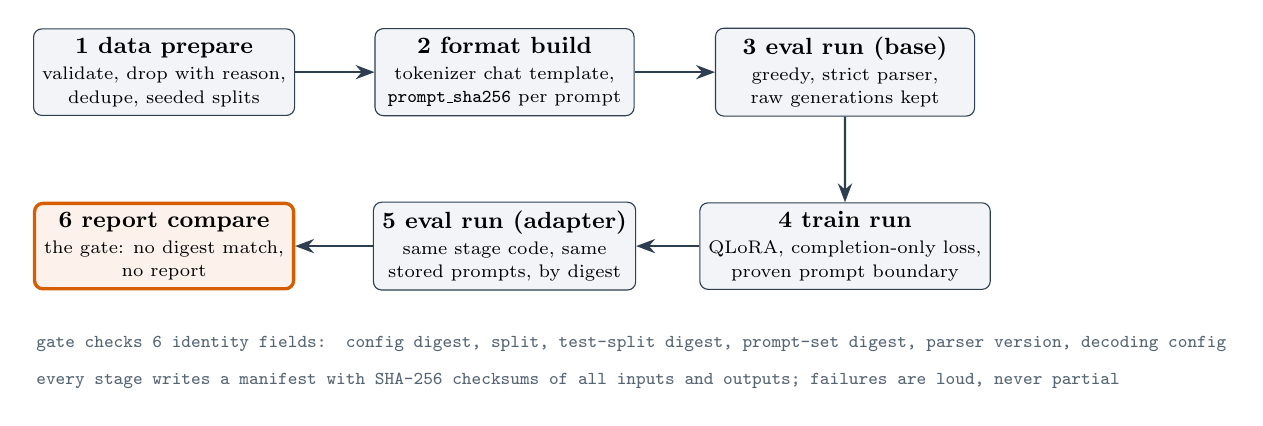
\begin{tikzpicture}[
      scale=0.94, every node/.style={transform shape},
      st/.style={draw=somink, fill=sompale, rounded corners=3pt, align=center,
                 minimum width=3.5cm, minimum height=1.05cm, font=\small},
      gate/.style={draw=somverm, very thick, fill=somverm!8, rounded corners=3pt, align=center,
                 minimum width=3.5cm, minimum height=1.05cm, font=\small},
      art/.style={font=\scriptsize\ttfamily, text=somink!80, align=left},
      arr/.style={-{Stealth[length=2.4mm]}, thick, somink}]
    \node[st]  (s1) at (0,0)     {\textbf{1 data prepare}\\[-1pt]\scriptsize validate, drop with reason,\\[-2pt]\scriptsize dedupe, seeded splits};
    \node[st]  (s2) at (4.6,0)   {\textbf{2 format build}\\[-1pt]\scriptsize tokenizer chat template,\\[-2pt]\scriptsize \texttt{prompt\_sha256} per prompt};
    \node[st]  (s3) at (9.2,0)   {\textbf{3 eval run (base)}\\[-1pt]\scriptsize greedy, strict parser,\\[-2pt]\scriptsize raw generations kept};
    \node[st]  (s4) at (9.2,-2.35) {\textbf{4 train run}\\[-1pt]\scriptsize QLoRA, completion-only loss,\\[-2pt]\scriptsize proven prompt boundary};
    \node[st]  (s5) at (4.6,-2.35) {\textbf{5 eval run (adapter)}\\[-1pt]\scriptsize same stage code, same\\[-2pt]\scriptsize stored prompts, by digest};
    \node[gate](s6) at (0,-2.35)  {\textbf{6 report compare}\\[-1pt]\scriptsize the gate: no digest match,\\[-2pt]\scriptsize no report};
    \draw[arr] (s1) -- (s2);
    \draw[arr] (s2) -- (s3);
    \draw[arr] (s3) -- (s4);
    \draw[arr] (s4) -- (s5);
    \draw[arr] (s5) -- (s6);
    \node[art, anchor=north west] at (-1.85,-3.45)
      {gate checks 6 identity fields: config digest, split, test-split digest, prompt-set digest, parser version, decoding config};
    \node[art, anchor=north west] at (-1.85,-3.95)
      {every stage writes a manifest with SHA-256 checksums of all inputs and outputs; failures are loud, never partial};
  \end{tikzpicture}
  \caption{The six-stage pipeline. Stages communicate only through schema-versioned files under one artifact root; there is no hidden state. Base and adapter evaluation are the same stage run twice, so no separate baseline script can drift. The comparison gate (stage 6) converts the one failure mode you cannot see, an invalid comparison, into one you cannot miss: a refused report.}
  \label{fig:pipeline}
\end{figure}

\sommelier{} is a staged command-line pipeline (Figure~\ref{fig:pipeline}): data preparation, chat formatting, baseline evaluation, QLoRA training, adapter evaluation, and comparison. The architecture rule is that stages communicate only through schema-versioned files under an artifact root; every transition writes a manifest listing its inputs and outputs with paths, schema versions, sizes, and SHA-256 digests. A zipped run directory handed to a stranger contains everything needed to audit the run: which commit, which resolved config, which inputs, and whether each stage finished. There is no database and no tracking service in the provenance path; evidence for a public claim has to travel with the claim. The pipeline's core never imports GPU libraries (\texttt{import sommelier} touches neither \texttt{torch} nor CUDA, enforced by a CI test that walks every module in a clean interpreter), and the data and formatting stages run on a laptop in fixture mode with no accounts and no downloads, so CI never needs hardware. This section describes the design decisions that make the measurement trustworthy; each was paid for in convenience.

\paragraph{Determinism as a contract.}
A run is driven by one YAML file, validated into a typed schema that rejects unknown keys: a misspelled hyperparameter is an error, not a silent default. The validated config is written back as \texttt{config.resolved.yaml}, and the SHA-256 of that file becomes the config digest stamped into every stage manifest and evaluation report. Model, tokenizer, and dataset revisions are required config fields with no defaults, because ``latest'' is not a reproducible input. Splits are seeded (seed 42 throughout) and deduplication runs before splitting, so a duplicated query cannot sit on both sides of the train/test boundary by construction; disjointness is re-asserted afterwards by intersecting hash sets. All structured values that feed a digest or a comparison use one canonical JSON form (sorted keys, compact separators), because without it every digest would measure key order instead of content. Determinism claims cover preparation, formatting, and evaluation; GPU training is explicitly not claimed to be bit-reproducible. The guarantee that matters is different: whatever adapter a run produced is scored under exactly the gate-checked conditions against a base model scored under the same conditions.

\paragraph{The comparison gate.}
Stage six refuses to write \texttt{comparison\_report.json} unless the base and adapter evaluation reports agree on six identity fields: config digest, split name, test-split digest, ordered prompt-set digest, parser version, and the exact decoding dictionary. It additionally re-hashes the run's own resolved config so a report cannot be smuggled in from a different run. A mismatch is an error naming the differing field, never a warning: a warning would be forgotten in a log while the report looked authoritative. The design intent is compressed in one sentence from the project documentation: the existence of the comparison report is itself the proof that the identity checks passed.

\paragraph{Evaluation that never repairs.}
The parser (\texttt{sommelier.parser.v1}) extracts the first balanced JSON span from the generation and accepts exactly one shape: an object with keys \texttt{name} (non-empty string) and \texttt{arguments} (object), or a one-element array of such an object. Nothing inside the span is repaired. Every generation receives one of four statuses (\texttt{ok}, \texttt{no\_json}, \texttt{invalid\_json}, \texttt{invalid\_shape}), and parse failures count against every metric: the denominators are always the full test split. A lenient parser would measure ``model plus repair heuristics,'' and since producing valid structure is itself one of our metrics, repair would erase part of exactly the signal we care about. Five metrics are computed, each stored with its numerator and denominator so any rate can be recomputed without trusting a float: valid-JSON rate, function-name accuracy, argument exact match (canonical-JSON equality), micro-averaged argument F1 over flattened argument path/value pairs, and full-call exact match, the strictest bar and the one to read as ``the model produced the right call.'' Raw generations are retained for every prompt, including failures, inside the complete run artifact root; a holder of that bundle can re-run the parser. The published v1/v2 repositories omit those files.

\paragraph{Training that proves its objective.}
Training uses completion-only loss: every prompt token is masked, and gradient flows only through the target, the canonical JSON of the gold call. The formatting stage fails unless the rendered full text begins with the prompt text, and the training collator re-proves the boundary at the token level for every example, verifying that tokenizing the full text yields the tokenization of the prompt as a strict prefix. If a tokenizer merges tokens across the boundary, training stops rather than silently fall back to full-sequence loss, because a failed run costs a rerun while an invisible objective change costs the comparison. Hyperparameters are never adjusted at runtime: an out-of-memory failure surfaces as an error quoting the exact config fields to change, since auto-tuning would let two runs with the same config digest train under different effective settings. In the project's phrasing, auto-tuning turns the config from a record into a suggestion.

\paragraph{Data policy with counted drops.}
Preparation treats every raw row as untrusted input and either yields a typed example or drops the row under the first failing reason from a closed, ordered list of sixteen. Two reasons are policy rather than quality: \texttt{multi\_call\_answer} (the v1 contract trains and scores exactly one call per request; Section~\ref{sec:recipes} explains why) and \texttt{duplicate\_query}. The remaining quality checks all counted zero on the recorded dataset revision, which is itself a useful, published fact about the source data.

\paragraph{Paired languages by construction.}
A config can declare one dataset source per language. Exactly one source is the root; every other source is paired row by row, naming its root example by identifier, inheriting the root's split assignment, and required to carry byte-identical tool schemas and gold answers. Violations are dropped under their own counted reasons. This turns ``the translation cannot contaminate the test set'' and ``the gap isolates query language as the only moving variable'' from good intentions into schema-checked invariants. The translator sits outside the six stages as a dataset production tool: it translates only the query, audits every output against protected spans (gold argument values that appear verbatim in the English query, matched with alphanumeric boundaries so a protected \texttt{2} is not satisfied by \texttt{2026}), retries twice with the rejection appended as feedback, and drops the pair with a counted reason if the audit still fails.

\paragraph{Release gates as code.}
Publication is gated by a preflight that machine-checks eight conditions, including the presence of license files, third-party notices covering the exact configured base model and dataset, the ``Built with Llama'' derived-artifact notice, an explicit human acknowledgment of the base-model license (an environment variable whose value must equal the base model identifier), a dependency lock, and a clean secret scan of the artifact tree. The preflight writes its evidence file before raising on failure, so even a refused release leaves a record.

\section{Experimental setup}
\label{sec:setup}

\paragraph{Base model and adapter.}
The base is \basemodel{}~\citep{bercovich2025llamanemotron}, an 8.03-billion-parameter dense decoder derived from Llama~3.1~8B~Instruct~\citep{grattafiori2024llama3}, already post-trained by NVIDIA for reasoning, code, and tool calling, with a 128k context window. We train LoRA adapters~\citep{hu2021lora} under the QLoRA recipe~\citep{dettmers2023qlora}: the frozen base is quantized to NF4 4-bit (double quantization, bfloat16 compute), and rank-16 adapters with $\alpha{=}32$ and dropout 0.05 attach to all seven linear projections of each of the 32 blocks, following the QLoRA finding that adapting every linear layer recovers full fine-tuning quality. The adapter totals 448 tensors and 41{,}943{,}040 trainable parameters, 0.52\% of the base, 168~MB on disk in float32. The $B$ matrices initialize to zero, so the untrained adapter is exactly a no-op: measured improvement is attributable to training alone. The adapter is never merged into the base; the separation is the evidence, since the base stays pinned by revision and the adapter is the entire diff. The stack is Transformers~\citep{wolf2019transformers}, PEFT~\citep{mangrulkar2022peft}, and bitsandbytes~\citep{dettmers2022llmint8}, with pinned versions recorded per run (reference run: torch 2.12.1, transformers 5.12.1, peft 0.19.1, bitsandbytes 0.49.2).

\paragraph{Data.}
The source is \texttt{Salesforce/xlam-function-calling-60k}~\citep{liu2024apigen}, 60{,}000 query/tools/answers rows generated and execution-verified by the APIGen pipeline over 3{,}673 APIs. Preparation kept 28{,}461 valid single-call rows (dropping 31{,}539, or 52.6\%, as multi-call by declared scope), deduplicated to 26{,}735, and drew seeded splits of 15{,}000 train, 1{,}000 validation, and 1{,}000 test. The exact split rows are published,\footnote{\texttt{huggingface.co/datasets/abdelstark/sommelier-xlam-single-call-splits} (en) and \texttt{...-fr} (fr), both CC-BY-4.0.} so verifying our results does not depend on upstream revision stability. For turn two, constrained translation (Mistral-Nemo-Instruct-2407~\citep{mistral2024nemo}, greedy, served with vLLM~\citep{kwon2023vllm}, pinned and recorded in the run manifest; no proprietary API in the loop) produced French variants of the selected rows: of 17{,}000, 14{,}936 pairs survived the audits (2{,}011 lost a protected span, 53 came back untranslated), yielding 13{,}113 French training rows and 879 French test pairs that inherit their sources' splits.

\paragraph{Protocol.}
Both runs share one training recipe: 2 epochs, per-device batch 4 with gradient accumulation 4 (effective 16), learning rate $2 \times 10^{-4}$ with cosine schedule and 3\% warmup, sequence budget 4{,}096 tokens, completion-only loss. Every rendered training sequence is audited against the budget immediately after formatting, per language. Evaluation generates one completion per held-out prompt with greedy decoding (temperature 0.0, sampling disabled, at most 512 new tokens), enforced rather than coerced: a config requesting anything else fails before a token is generated. The system prompt is English for every language by design, so the query language is the only moving variable; instruction-language effects are a separate, unmeasured experiment. All runs execute on a single rented L40S (44~GiB) through a remote driver on Modal that exports the pinned dataset in-container, chains the six stages with per-stage GPU cleanup, and commits artifacts to a volume after every stage.

\paragraph{Cost accounting.}
The run records report cost as unavailable because the provider exposed no billing data to the run itself. From the maintainer's private billing console, outside the checksummed run record, turn one billed about eight dollars for roughly 3.7 GPU hours end to end; turn two's roughly sixteen-dollar figure extrapolates the same observed rate over about seven recorded GPU hours. Failed attempts along the way (including a serving crash-loop, Section~\ref{sec:recipes}) were observed to cost about as much again as turn one. These cost figures are operational context, not independently verifiable public run evidence.

\section{Turn one: teaching the call in English}
\label{sec:turn1}

\begin{table}[t]
  \caption{Turn one (run \texttt{nemotron-8b-full-3}): base versus v1 adapter on 1{,}000 held-out English prompts, greedy decoding, strict parser, parse failures counted against every metric. Values quoted with their counts exactly as the comparison report records them. Argument F1 is micro-averaged over flattened argument pairs, so its counts are not per-example.}
  \label{tab:v1}
  \centering
  \small
  \begin{tabular}{lccc}
    \toprule
    Metric & Base & Adapter & $\Delta$ \\
    \midrule
    Valid JSON rate & 0.9160 \scriptsize(916/1000) & \textbf{1.0000} \scriptsize(1000/1000) & $+0.0840$ \\
    Function name accuracy & 0.9110 \scriptsize(911/1000) & \textbf{0.9960} \scriptsize(996/1000) & $+0.0850$ \\
    Argument exact match & 0.7070 \scriptsize(707/1000) & \textbf{0.8760} \scriptsize(876/1000) & $+0.1690$ \\
    Argument F1 & 0.7569 \scriptsize(3858/5097) & \textbf{0.9291} \scriptsize(5122/5513) & $+0.1722$ \\
    Full-call exact match & 0.7050 \scriptsize(705/1000) & \textbf{0.8740} \scriptsize(874/1000) & $+0.1690$ \\
    \bottomrule
  \end{tabular}
\end{table}

Table~\ref{tab:v1} and Figure~\ref{fig:results}a give the headline result. Training took 10{,}996 seconds (just over three hours, 1{,}876 optimizer steps, about 5.9~s each) at 26{,}306~MiB peak GPU memory; the two 1{,}000-prompt evaluations took 13.7 and 15.4 minutes. Training loss fell from 1.085 to 0.042 over 16{,}668{,}132 seen tokens, with validation loss 0.038 at the epoch boundary and 0.030 at the end.

Three readings of the table. First, structural validity saturates: the adapter produced a schema-valid single tool call on all 1{,}000 prompts, against 916 for the base, whose 84 failures split into 64 \texttt{invalid\_shape} (fifty of which were bare argument dictionaries missing the name/arguments wrapper), 11 \texttt{invalid\_json}, and 9 \texttt{no\_json}. Second, function naming is nearly solved (996/1000). Third, the residual errors are argument construction: 996 correct names against 876 exact argument matches. Reading the raw generations shows some of these are genuine mistakes and others are semantically right values in the wrong surface form, which canonical-JSON equality scores as wrong for both models equally; the absolute numbers are conservative and the deltas are the point. The per-example transition matrix (Appendix~\ref{app:transitions}) adds the honest detail aggregates hide: of the base's 84 parse failures, the adapter converts 64 into exact calls, while 29 prompts regress from an exact base call to a non-exact adapter call. Both directions are counted; nothing is netted away.

An objection worth pre-empting: constrained decoding could get 100\% valid JSON out of the base model without any training, and grammar-guided generation works. What constrained decoding cannot supply is the jump from 0.705 to 0.874 in full-call exact match. That delta is the model getting better at choosing the right function and constructing the right arguments, not at emitting parseable syntax.

\begin{figure}[t]
  \centering
  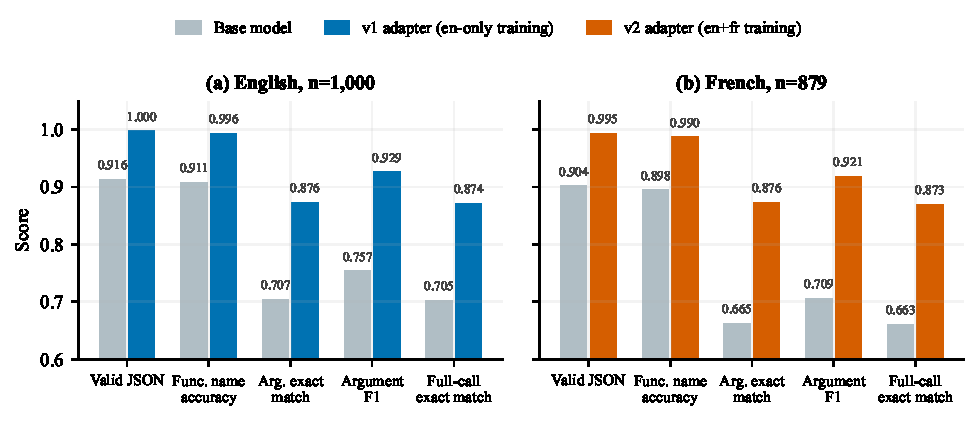
\includegraphics[width=\linewidth]{figures/fig_results.pdf}
  \caption{Base versus adapter across the five metrics. (a) English slice of turn one (run \texttt{nemotron-8b-full-3}, $n{=}1{,}000$). (b) French slice of turn two (run \texttt{nemotron-8b-fr-full-4}, $n{=}879$). Parse failures count against every metric; exact-match scoring is canonical-JSON equality. Exact numerators and denominators in Tables~\ref{tab:v1} and~\ref{tab:v2}.}
  \label{fig:results}
\end{figure}

\section{Turn two: closing the language gap with the flywheel's own output}
\label{sec:turn2}

The question turn one left open is the one our simulated French company cares about most: does the capability survive translation to the users' language? Turn two answers it with a single-variable experiment. Same base model, same hyperparameters, same seed, same pipeline; the only change is the training data, which adds a constrained-translation French pair for nearly every selected English row (the pairing runs short where the gold contract rejects translation; Section~\ref{sec:setup} carries the exact drop accounting). The English evaluation prompts are byte-identical to turn one's by digest, so the three models we compare (base, v1 adapter, v2 adapter) stand on the same measurement surface.

\begin{table}[t]
  \caption{Turn two (run \texttt{nemotron-8b-fr-full-4}): base versus v2 adapter on both evaluation slices. The English prompt-set digest is identical to turn one's. French gold answers and tool schemas are byte-identical to their English sources by construction.}
  \label{tab:v2}
  \centering
  \small
  \begin{tabular}{lcccccc}
    \toprule
    & \multicolumn{3}{c}{English ($n{=}1{,}000$)} & \multicolumn{3}{c}{French ($n{=}879$)} \\
    \cmidrule(lr){2-4}\cmidrule(lr){5-7}
    Metric & Base & v2 & $\Delta$ & Base & v2 & $\Delta$ \\
    \midrule
    Valid JSON rate & 0.9160 & \textbf{0.9970} & $+0.0810$ & 0.9044 & \textbf{0.9954} & $+0.0910$ \\
    Function name accuracy & 0.9110 & \textbf{0.9930} & $+0.0820$ & 0.8976 & \textbf{0.9898} & $+0.0922$ \\
    Argument exact match & 0.7070 & \textbf{0.8730} & $+0.1660$ & 0.6655 & \textbf{0.8760} & $+0.2105$ \\
    Argument F1 & 0.7569 & \textbf{0.9211} & $+0.1642$ & 0.7091 & \textbf{0.9208} & $+0.2117$ \\
    Full-call exact match & 0.7050 & \textbf{0.8700} & $+0.1650$ & 0.6633 & \textbf{0.8726} & $+0.2093$ \\
    \bottomrule
  \end{tabular}
\end{table}

\begin{figure}[t]
  \centering
  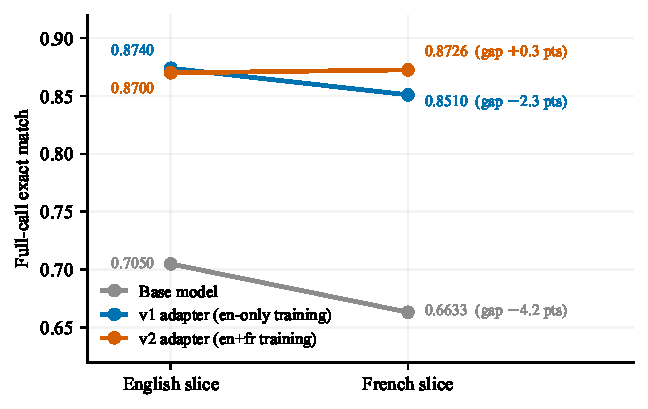
\includegraphics[width=0.72\linewidth]{figures/fig_language_gap.pdf}
  \caption{The language gap, measured three ways: full-call exact match on the English and French slices for the base model, the v1 adapter (English-only training), and the v2 adapter (mixed training). English-only fine-tuning transfers most of its gains to French unseen; the machine-translated French training data closes the remaining gap to measurement noise.}
  \label{fig:gap}
\end{figure}

Table~\ref{tab:v2} and Figures~\ref{fig:results}b and~\ref{fig:gap} carry three findings, stated plainly.

\textbf{The language tax is real and concentrated.} The base model pays 4.2 points of full-call exact match on French input (0.7050 English against 0.6633 French). The penalty concentrates in argument construction: argument exact match drops from 0.707 to 0.666 while name accuracy moves far less. Same tools, same gold calls, same parser; only the query language changed.

\textbf{Format discipline transfers across languages for free.} The v1 adapter, trained without a single French example, lifts French full-call exact match by 18.8 points (0.663 to 0.851), narrowing the gap from 4.2 to 2.3 points. Cross-lingual generalization from finetuning is a documented phenomenon~\citep{muennighoff2022crosslingual}; measuring it on strict, execution-shaped tool calls, under a parser that never repairs, makes the practical version of the claim concrete: most of what fine-tuning teaches here is a language-independent contract.

\textbf{The flywheel's own output narrows the displayed marginal difference.} With the 13{,}113 machine-translated pairs mixed in, the complete French and English slices differ by at most a third of a point ($+0.3$ points on full-call exact match). Those slices contain 879 and 1{,}000 rows, so this is a descriptive marginal comparison, not an exact-pair language effect; the v2 artifact predates the paired interval now required by v3. The training data for this turn required no manual annotation: it was manufactured from turn one's published artifacts by an open, pinned translator under a byte-identity contract, with every rejected pair counted (Section~\ref{sec:setup}). The cost, reported rather than hidden: the v2 adapter's English slice sits 0.3 to 0.8 points below the v1 reference depending on the metric (full-call 0.8700 against 0.8740). At $n{=}1{,}000$ this is within one standard error, and with one seed we cannot decide between noise and a small capacity price for bilingual coverage. We state it in those terms because a number that does not admit its uncertainty is an advertisement.

\section{Recipes: what only real runs teach}
\label{sec:recipes}

The pipeline's test suite (roughly 300 tests at the time, 390 today: golden prompt fixtures, parser and metric regression snapshots, split-leakage property tests, an import-discipline gate) was green before the first real GPU run, and the first three remote runs still failed. This section is the educational core of the paper: the specific failures, what each cost, and the general recipe each one taught. None are exotic. They are what the gap between passing tests and honest measurement looks like in a stack whose libraries move monthly.

\paragraph{Recipe 1: your evaluation can be wrong in a direction that looks exactly like a model failure.}
The first real smoke run showed the adapter \emph{worse} than the base on every metric, with valid JSON collapsing from 95\% to 40\%. The honest conclusion appeared to be that fine-tuning hurt. Reading the raw generations showed the opposite: the adapter had learned its training format perfectly, reproducing complete gold answers byte for byte. The problem was the evaluation contract. The source dataset is 52.6\% multi-call rows; against a single-call parser, the base model's habit of emitting multiple loose JSON objects let the parser extract the first balanced span, which matched the first gold call (full credit), while the adapter's faithful multi-call array was rejected as \texttt{invalid\_shape} (zero). A model could emit the byte-exact gold target and score zero while a model that ignored half the task scored full marks. The fix was to make the data agree with the contract: preparation drops multi-call rows under a declared, counted reason, so training targets, parser, and metrics describe the same task. The general form deserves tattooing on every evaluation harness: \emph{a metric can be wrong in a direction you did not anticipate, and it will look exactly like a model failure. The only defense is keeping raw generations and actually reading them.} This is also why the flywheel argument of Section~\ref{sec:flywheel} insists on retained generations: an unauditable turn would have baked this inversion into every subsequent turn.

\paragraph{Recipe 2: the quiet failures ship with the frameworks.}
Five failures that no green test caught, each now guarded by an explicit check. (i)~\emph{Double BOS}: the rendered chat template already contains the begin-of-text token; tokenizing it again with \texttt{add\_special\_tokens=True} silently duplicated it, corrupting both models identically, so no comparison test could see it. (ii)~\emph{The trainer ate the collator's columns}: recent Transformers wraps custom collators in a \texttt{RemoveColumnsCollator} that strips features absent from the model's forward signature, including the prompt and full text the completion-only collator needs; \texttt{remove\_unused\_columns=False} is load-bearing. (iii)~\emph{Library defaults drift}: gradient checkpointing that an earlier PEFT k-bit preparation enabled was no longer active under the current library combination, and batch 8 ran a 44~GiB L40S out of memory. Explicit \texttt{gradient\_checkpointing=True} plus half the micro-batch at the same effective batch brought peak memory to 26~GiB and, counterintuitively, faster steps (5.4~s against 8.5~s). (iv)~\emph{Real data has a longer tail than you think}: two prompts in 16{,}000 exceeded the original 2{,}048-token budget (real rows render to 2{,}166 tokens). The pipeline now audits every rendered sequence, per language, immediately after formatting, so a budget violation costs seconds instead of failing training forty minutes in, after the baseline evaluation already spent its GPU time. (v)~\emph{vLLM needs nvcc}: serving crash-looped for hours with the engine dying before it could log, because vLLM JIT-compiles kernels at startup and slim images lack the CUDA toolkit; the devel base image fixed it, and a foreground-diagnostics entrypoint now makes that class of silent failure cost one focused run.

\paragraph{Recipe 3: translation pipelines fail on the details your contract protects.}
The constrained translator initially discarded perfectly good pairs because a French model writes \texttt{0,5} where the gold answer requires \texttt{0.5}; protected numeric spans broke on the decimal comma. Deterministic normalization (rewrite the comma variant back only when the protected dot form is missing and the comma form is present at alphanumeric boundaries) recovered them, and is tested. Related guards that earned their place: span matching is boundary-aware so short and numeric spans cannot be satisfied by substrings of larger tokens; completions that hit the token budget are treated as empty rather than audited, because a truncated translation can pass a span audit with a garbled tail; and progress is checkpointed per row, keyed by the source query digest, so an interrupted run resumes without grafting stale translations onto changed inputs.

\paragraph{Recipe 4: grade your evidence, and make the grades unmistakable.}
Every claim in this paper comes from the top rung of a three-rung ladder the project enforces. Local tests and fixture mode prove the machinery with no GPU. Smoke runs execute the full six-stage chain on a GPU at 100/20/20 examples in about half an hour; they carry a \texttt{smoke-} run-identifier prefix and an explicit ``Evidence class: smoke run'' line in their reports, because a 20-prompt evaluation is a plumbing check, not a measurement, and the report format exists so it cannot be mistaken for one. Full runs at 15{,}000/1{,}000/1{,}000 produce the quotable numbers. The corollary recipe: failures should be loud and diagnostic. Every expected error names the config fields at fault and maps to a documented exit code; nothing retries with altered settings; and no stage anywhere is permitted to substitute a plausible number for a refused one.

\section{Related work}
\label{sec:related}

\paragraph{Tool use and function calling.}
Toolformer taught models to invoke tools from self-supervised data~\citep{schick2023toolformer}; Gorilla fine-tuned open models for large API surfaces~\citep{patil2023gorilla}; ToolLLM scaled instruction data over thousands of real APIs~\citep{qin2023toolllm}. Our training data comes from APIGen's execution-verified generation pipeline~\citep{liu2024apigen}. The Berkeley Function Calling Leaderboard~\citep{patil2025bfcl} is the standard external benchmark for this skill; we deliberately rank nothing against it. \sommelier's claim is complementary and narrower: not ``this model is better than that model'' but ``this adapter beats this base under provably identical conditions,'' the comparison a team actually needs when deciding whether to own its tool caller.

\paragraph{Parameter-efficient adaptation.}
LoRA~\citep{hu2021lora} and QLoRA~\citep{dettmers2023qlora} supply the economics that make the sovereignty argument work, with LLM.int8 underpinning the quantized stack~\citep{dettmers2022llmint8}, implemented via PEFT~\citep{mangrulkar2022peft} and Transformers~\citep{wolf2019transformers}; serving uses vLLM~\citep{kwon2023vllm}. Our contribution on top of these methods is not algorithmic; it is the evidentiary machinery around them.

\paragraph{Multilingual adaptation.}
Okapi~\citep{lai2023okapi} and the Aya model and dataset~\citep{ustun2024aya,singh2024ayadataset} established multilingual instruction tuning on open models at breadth. Turn two differs in shape: a depth-first, single-language extension manufactured from the pipeline's own published artifacts under a byte-identity contract. Inside each surviving pair, the query language is the designed text difference while tools and gold calls remain identical; the published v2 cross-language table nevertheless compares unequal complete cohorts and is therefore marginal rather than an exact paired effect.

\paragraph{ML systems and documentation.}
Hidden technical debt~\citep{sculley2015hidden} named the failure class our gates exist to prevent. Model cards~\citep{mitchell2019modelcards} and datasheets~\citep{gebru2021datasheets} standardized documentation of models and datasets; \sommelier{} extends the same ethic to the run itself, treating the comparison report, with its digests, counts, and claim boundaries, as the unit of publishable evidence. The data flywheel framing comes from NVIDIA~\citep{nvidia2026flywheel,arunagiri2025flywheel,verma2025flywheel}; our position sharpens it with auditability as the load-bearing requirement, and our sovereignty framing engages the emerging literature~\citep{singh2025sovereignai,srivastava2024digitalsovereignty,europeanunion2024aiact}.

\section{Limitations}
\label{sec:limitations}

The claim boundaries are part of the result, and the pipeline prints them into every report. All metrics measure schema-valid \emph{single} tool calls on held-out splits of one dataset family; multi-call planning, multi-turn tool use, tool execution, and retry logic are out of scope, and 52.6\% of the source rows were filtered by that scope decision. Argument scoring is exact canonical-JSON equality: semantically equivalent but differently formatted values count as wrong for both models, so absolute numbers are conservative even though deltas stay fair. Each turn is one run with one seed; the v2-versus-v1 English difference (0.3 to 0.8 points) is within one standard error and stays undecided. The French test set is machine-translated and sample-reviewed, not natively authored; 12.1\% of test pairs were excluded because their gold arguments embed English text from the query, biasing the slice toward language-neutral arguments; and the system prompt remains English for both languages, so instruction-language effects are unmeasured. The adapter is trained against the NF4-quantized base but evaluated and served against the bfloat16 base (the original QLoRA recipe on one side, a deployment choice on the other); both sides of every comparison use the same bfloat16 base, so the deltas stay internally consistent. Out-of-distribution tool schemas degrade the adapter visibly, as parse failures, because it learned the source dataset's flat parameter style. Nothing here ranks the model against any public benchmark or hosted model, and none of it is a claim of production readiness. Finally, the eight-dollar figure is a maintainer billing-console observation and the sixteen-dollar figure an extrapolation at the same observed rate; the run records themselves report cost as unavailable rather than estimated.

\paragraph{Public evidence boundary.}
The published v1/v2 repositories contain exact splits, adapters, and aggregate evaluation/comparison reports with counts and digests, but not the raw generation files retained by the original runs. The reported aggregate rates can therefore be checked against their public numerators and denominators, while independent row-wise rescoring requires reproducing the run. Neither cost figure is independently verifiable from a public billing artifact.

\section{Conclusion}
\label{sec:conclusion}

We set out to answer a question a thousand teams are asking: can a small open model, post-trained cheaply on your own schemas, carry the tool-calling load of an agentic product, and can you prove it with numbers instead of vibes? Two turns of an auditable flywheel later, the answer is concrete. Three GPU hours accompanied a maintainer-observed bill of about eight dollars and a 16.9-point lift in full-call exactness with structural validity saturated. In the second turn, the historical marginal French and English slice values differ by a third of a point; an exact paired parity claim is withheld because those slices contain different cohorts. Its roughly sixteen-dollar cost is an extrapolation from the first run's observed rate, not a second billing record. The model learned the sommelier's job quickly. Building the instruments that make the measurement trustworthy, the digests, the gates, the counted drops, the parser that refuses to help, took most of the effort, and that ratio is, we suspect, the honest shape of applied AI work.

The position we hope travels: turn your own flywheel, and make every turn auditable. The first property makes you sovereign; the second keeps you honest, and the loop compounds only if it is both. The pipeline, exact splits, adapters, and aggregate reports are public~\citep{bakhta2026sommelier}; those reports expose counts and identity digests but the published v1/v2 repositories omit raw generations, so row-wise rescoring requires reproduction. Steal the comparison gate and the boundary-proving collator first; argue with the parser; and if you disagree with an aggregate, the public report is where to start.

\begin{ack}
This work builds on NVIDIA's open Nemotron stack (weights, tooling, and published data recipes) and on the Hugging Face open-source ecosystem. The paper was prepared with AI writing and analysis assistance. Metric and runtime numbers were cross-checked against published run reports; cost figures retain their maintainer-observation and extrapolation labels.
\end{ack}

\bibliographystyle{plainnat}
\bibliography{references}

\appendix

\section{Run identity}
\label{app:identity}

Both runs are anchored by digests that the comparison gate verified before their reports could exist. Anyone reproducing a run can check their digests against these.

\begin{table}[h]
  \caption{Published run identities.}
  \label{tab:identity}
  \centering
  \scriptsize
  \begin{tabular}{lll}
    \toprule
    Field & Turn one & Turn two \\
    \midrule
    Run ID & \texttt{nemotron-8b-full-3} & \texttt{nemotron-8b-fr-full-4} \\
    Executed & 2026-07-02 & 2026-07-06 \\
    Evidence class & full run & full run \\
    Config digest & \texttt{3a8fb0d8b4f5b4c6\ldots} & \texttt{87a6c067167d801d\ldots} \\
    Test split digest & \texttt{db8dd82f2a295774\ldots} & \texttt{11267f2e2e6293b6\ldots} \\
    Prompt set digest (en) & \texttt{a0da8fa28835a329\ldots} & \texttt{a0da8fa28835a329\ldots} (identical) \\
    Prompt set digest (fr) & & \texttt{b6111339b6dd6d6a\ldots} \\
    Parser & \texttt{sommelier.parser.v1} & \texttt{sommelier.parser.v1} \\
    Decoding & \multicolumn{2}{l}{\texttt{\{"do\_sample": false, "max\_new\_tokens": 512, "temperature": 0.0\}}} \\
    Peak GPU memory & 26{,}306 MiB & 26{,}369 MiB \\
    \bottomrule
  \end{tabular}
\end{table}

Full digests, per-slice aggregate evaluation reports, and runtime metadata are published under \texttt{reports/} in the adapter repositories on the Hugging Face Hub. The reports reference raw-generation paths from the original run artifact roots, but those files are not present in the published repositories:
\begin{itemize}
  \item v1: \texttt{abdelstark/llama-3.1-nemotron-nano-8b-xlam-tool-calling-lora}
  \item v2: \texttt{abdelstark/llama-3.1-nemotron-nano-8b-xlam-tool-calling-fr-en-lora}
\end{itemize}

\section{Runtime}
\label{app:runtime}

\begin{table}[h]
  \caption{Per-stage wall clock, from each run's \texttt{runtime\_metadata.json}. Turn two evaluates two slices per model (1{,}879 prompts per evaluation) and trains on 28{,}113 rows (3{,}516 optimizer steps).}
  \label{tab:runtime}
  \centering
  \small
  \begin{tabular}{lrr}
    \toprule
    Stage & Turn one (s) & Turn two (s) \\
    \midrule
    data prepare & 5.6 & 8.1 \\
    format build & 16.9 & 30.6 \\
    eval run (base) & 823.5 & 1{,}805.2 \\
    train run & 10{,}996.0 & 20{,}540.3 \\
    eval run (adapter) & 923.4 & 2{,}835.1 \\
    report compare & 1.3 & 1.1 \\
    \bottomrule
  \end{tabular}
\end{table}

The per-language sequence audit measured French rows at nearly identical token lengths to English (max 2{,}174 against 2{,}166, 95th percentile 711 against 716, budget 4{,}096), so the bilingual run's extra compute is purely its extra rows.

\section{Base-to-adapter transitions (English, turn one)}
\label{app:transitions}

Per-prompt outcome transitions between base and v1 adapter on the 1{,}000 English prompts. Outcomes: exact (full-call exact match), args\_mismatch (right name, wrong arguments), name\_mismatch, and the three parse-failure statuses. The authors derived this matrix from the retained local v1 generations; the public aggregate reports verify its row and column totals only indirectly and do not contain the row-level files needed to reconstruct it independently.

\begin{table}[h]
  \caption{Transition counts, base outcome $\rightarrow$ adapter outcome ($n{=}1{,}000$). Cells with zero count omitted.}
  \label{tab:transitions}
  \centering
  \small
  \begin{tabular}{lr@{\qquad}lr}
    \toprule
    Transition & Count & Transition & Count \\
    \midrule
    exact $\rightarrow$ exact & 676 & no\_json $\rightarrow$ exact & 8 \\
    args\_mismatch $\rightarrow$ exact & 131 & name\_mismatch $\rightarrow$ exact & 3 \\
    args\_mismatch $\rightarrow$ args\_mismatch & 74 & invalid\_json $\rightarrow$ args\_mismatch & 3 \\
    invalid\_shape $\rightarrow$ exact & 48 & name\_mismatch $\rightarrow$ name\_mismatch & 2 \\
    exact $\rightarrow$ args\_mismatch & 28 & args\_mismatch $\rightarrow$ name\_mismatch & 1 \\
    invalid\_shape $\rightarrow$ args\_mismatch & 16 & no\_json $\rightarrow$ args\_mismatch & 1 \\
    invalid\_json $\rightarrow$ exact & 8 & exact $\rightarrow$ name\_mismatch & 1 \\
    \bottomrule
  \end{tabular}
\end{table}

Of the base's 84 parse failures, the adapter converts 64 into exact calls. The 29 regressions (base exact, adapter not) are real and counted.

\section{Reference configuration and reproduction}
\label{app:repro}

The full configuration behind both runs is \texttt{examples/config.full.yaml} in the repository; the key fields:

{\small
\begin{verbatim}
schema_version: sommelier.config.v2
project: {seed: 42}
model:
  base_model_id: nvidia/Llama-3.1-Nemotron-Nano-8B-v1
  base_model_revision: main        # pinned; required, no default
datasets:
  - {language: en, dataset_id: Salesforce/xlam-function-calling-60k}
  - {language: fr, dataset_id: abdelstark/sommelier-xlam-single-call-splits-fr,
     source_id_column: source_example_id}   # paired source
data: {n_train: 15000, n_validation: 1000, n_test: 1000}
train:
  epochs: 2
  per_device_batch_size: 4
  gradient_accumulation_steps: 4
  learning_rate: 2.0e-4
  scheduler: cosine
  warmup_ratio: 0.03
  max_sequence_length: 4096
  quantization: nf4-4bit
  compute_dtype: bfloat16
  lora_rank: 16
  lora_alpha: 32
  lora_dropout: 0.05
  target_modules: [q_proj, k_proj, v_proj, o_proj,
                   gate_proj, up_proj, down_proj]
eval: {temperature: 0.0, do_sample: false, max_new_tokens: 512}
remote: {gpu: L40S}
\end{verbatim}
}

Reproduction, from a clean checkout with Modal credentials (turn one, then turn two):

{\small
\begin{verbatim}
# turn one: English reference run
SOMMELIER_GPU=L40S SOMMELIER_TIMEOUT_SECONDS=28800 \
  uv run modal run --detach remote_pipeline.py \
  --config examples/config.full.yaml --mode full --max-rows 60000

# turn two: constrained translation, then the bilingual run
SOMMELIER_GPU=L40S SOMMELIER_TIMEOUT_SECONDS=14400 \
  uv run modal run --detach remote_translate.py \
  --config examples/config.full.yaml --run-id fr-translate-2
SOMMELIER_GPU=L40S SOMMELIER_TIMEOUT_SECONDS=36000 \
  uv run modal run --detach remote_pipeline.py \
  --config examples/config.full.yaml --mode full --max-rows 60000 \
  --translation-run-id fr-translate-2
\end{verbatim}
}

Local validation needs no GPU and no accounts: \texttt{uv sync --extra dev}, then \texttt{ruff}, \texttt{mypy}, the full \texttt{pytest} suite, config validation, and a fixture pipeline slice. Publication requires \texttt{sommelier release preflight} with the base-model license acknowledged by exact identifier. Reproduction uses the same splits and digest-bound protocol, but bit-identical generations across different GPUs and driver stacks are not guaranteed.

\end{document}
